%-----------------------------------------------------------------------------------------------------------------------------------------------%
%	The MIT License (MIT)
%
%	Copyright (c) 2019 Jan Küster
%
%	Permission is hereby granted, free of charge, to any person obtaining a copy
%	of this software and associated documentation files (the "Software"), to deal
%	in the Software without restriction, including without limitation the rights
%	to use, copy, modify, merge, publish, distribute, sublicense, and/or sell
%	copies of the Software, and to permit persons to whom the Software is
%	furnished to do so, subject to the following conditions:
%	
%	THE SOFTWARE IS PROVIDED "AS IS", WITHOUT WARRANTY OF ANY KIND, EXPRESS OR
%	IMPLIED, INCLUDING BUT NOT LIMITED TO THE WARRANTIES OF MERCHANTABILITY,
%	FITNESS FOR A PARTICULAR PURPOSE AND NONINFRINGEMENT. IN NO EVENT SHALL THE
%	AUTHORS OR COPYRIGHT HOLDERS BE LIABLE FOR ANY CLAIM, DAMAGES OR OTHER
%	LIABILITY, WHETHER IN AN ACTION OF CONTRACT, TORT OR OTHERWISE, ARISING FROM,
%	OUT OF OR IN CONNECTION WITH THE SOFTWARE OR THE USE OR OTHER DEALINGS IN
%	THE SOFTWARE.
%	
%
%-----------------------------------------------------------------------------------------------------------------------------------------------%


%============================================================================%
%
%	DOCUMENT DEFINITION
%
%============================================================================%

%we use article class because we want to fully customize the page and don't use a cv template
\documentclass[10pt,A4]{article}	


%----------------------------------------------------------------------------------------
%	ENCODING
%----------------------------------------------------------------------------------------

% we use utf8 since we want to build from any machine
\usepackage[utf8]{inputenc}		

%----------------------------------------------------------------------------------------
%	LOGIC
%----------------------------------------------------------------------------------------

% provides \isempty test
\usepackage{xstring, xifthen}

%----------------------------------------------------------------------------------------
%	FONT BASICS
%----------------------------------------------------------------------------------------

% some tex-live fonts - choose your own

%\usepackage[defaultsans]{droidsans}
%\usepackage[default]{comfortaa}
%\usepackage{cmbright}
\usepackage[default]{raleway}
%\usepackage{fetamont}
%\usepackage[default]{gillius}
%\usepackage[light,math]{iwona}
%\usepackage[thin]{roboto} 

% set font default
\renewcommand*\familydefault{\sfdefault} 	
\usepackage[T1]{fontenc}

% more font size definitions
\usepackage{moresize}

%----------------------------------------------------------------------------------------
%	FONT AWESOME ICONS
%---------------------------------------------------------------------------------------- 

% include the fontawesome icon set
\usepackage{fontawesome}

% use to vertically center content
% credits to: http://tex.stackexchange.com/questions/7219/how-to-vertically-center-two-images-next-to-each-other
\newcommand{\vcenteredinclude}[1]{\begingroup
\setbox0=\hbox{\includegraphics{#1}}%
\parbox{\wd0}{\box0}\endgroup}

% use to vertically center content
% credits to: http://tex.stackexchange.com/questions/7219/how-to-vertically-center-two-images-next-to-each-other
\newcommand*{\vcenteredhbox}[1]{\begingroup
\setbox0=\hbox{#1}\parbox{\wd0}{\box0}\endgroup}

% icon shortcut
\newcommand{\icon}[3] { 							
	\makebox(#2, #2){\textcolor{maincol}{\csname fa#1\endcsname}}
}	

% icon with text shortcut
\newcommand{\icontext}[4]{ 						
	\vcenteredhbox{\icon{#1}{#2}{#3}}  \hspace{2pt}  \parbox{0.9\mpwidth}{\textcolor{#4}{#3}}
}

% icon with website url
\newcommand{\iconhref}[5]{ 						
    \vcenteredhbox{\icon{#1}{#2}{#5}}  \hspace{2pt} \href{#4}{\textcolor{#5}{#3}}
}

% icon with email link
\newcommand{\iconemail}[5]{ 						
    \vcenteredhbox{\icon{#1}{#2}{#5}}  \hspace{2pt} \href{mailto:#4}{\textcolor{#5}{#3}}
}

%----------------------------------------------------------------------------------------
%	PAGE LAYOUT  DEFINITIONS
%----------------------------------------------------------------------------------------

% page outer frames (debug-only)
% \usepackage{showframe}		

% we use paracol to display breakable two columns
\usepackage{paracol}

% define page styles using geometry
\usepackage[a4paper]{geometry}

% remove all possible margins
\geometry{top=1cm, bottom=1cm, left=1cm, right=1cm}

\usepackage{fancyhdr}
\pagestyle{empty}

% space between header and content
% \setlength{\headheight}{0pt}

% indentation is zero
\setlength{\parindent}{0mm}

%----------------------------------------------------------------------------------------
%	TABLE /ARRAY DEFINITIONS
%---------------------------------------------------------------------------------------- 

% extended aligning of tabular cells
\usepackage{array}

% custom column right-align with fixed width
% use like p{size} but via x{size}
\newcolumntype{x}[1]{%
>{\raggedleft\hspace{0pt}}p{#1}}%


%----------------------------------------------------------------------------------------
%	GRAPHICS DEFINITIONS
%---------------------------------------------------------------------------------------- 

%for header image
\usepackage{graphicx}

% use this for floating figures
% \usepackage{wrapfig}
% \usepackage{float}
% \floatstyle{boxed} 
% \restylefloat{figure}

%for drawing graphics		
\usepackage{tikz}				
\usetikzlibrary{shapes, backgrounds,mindmap, trees}

%----------------------------------------------------------------------------------------
%	Color DEFINITIONS
%---------------------------------------------------------------------------------------- 
\usepackage{transparent}
\usepackage{color}

% primary color
\definecolor{maincol}{RGB}{ 225, 0, 0 }

% accent color, secondary
% \definecolor{accentcol}{RGB}{ 250, 150, 10 }

% dark color
\definecolor{darkcol}{RGB}{ 70, 70, 70 }

% light color
\definecolor{lightcol}{RGB}{245,245,245}


% Package for links, must be the last package used
\usepackage[hidelinks]{hyperref}

% returns minipage width minus two times \fboxsep
% to keep padding included in width calculations
% can also be used for other boxes / environments
\newcommand{\mpwidth}{\linewidth-\fboxsep-\fboxsep}
	


%============================================================================%
%
%	CV COMMANDS
%
%============================================================================%

%----------------------------------------------------------------------------------------
%	 CV LIST
%----------------------------------------------------------------------------------------

% renders a standard latex list but abstracts away the environment definition (begin/end)
\newcommand{\cvlist}[1] {
	\begin{itemize}{#1}\end{itemize}
}

%----------------------------------------------------------------------------------------
%	 CV TEXT
%----------------------------------------------------------------------------------------

% base class to wrap any text based stuff here. Renders like a paragraph.
% Allows complex commands to be passed, too.
% param 1: *any
\newcommand{\cvtext}[1] {
	\begin{tabular*}{1\mpwidth}{p{0.98\mpwidth}}
		\parbox{1\mpwidth}{#1}
	\end{tabular*}
}

%----------------------------------------------------------------------------------------
%	CV SECTION
%----------------------------------------------------------------------------------------

% Renders a a CV section headline with a nice underline in main color.
% param 1: section title
\newcommand{\cvsection}[1] {
	\vspace{14pt}
	\cvtext{
		\textbf{\LARGE{\textcolor{darkcol}{\uppercase{#1}}}}\\[-4pt]
		\textcolor{maincol}{ \rule{0.1\textwidth}{2pt} } \\
	}
}

%----------------------------------------------------------------------------------------
%	META SKILL
%----------------------------------------------------------------------------------------

% Renders a progress-bar to indicate a certain skill in percent.
% param 1: name of the skill / tech / etc.
% param 2: level (for example in years)
% param 3: percent, values range from 0 to 1
\newcommand{\cvskill}[3] {
	\begin{tabular*}{1\mpwidth}{p{0.72\mpwidth}  r}
 		\textcolor{black}{\textbf{#1}} & \textcolor{maincol}{#2}\\
	\end{tabular*}%
	
	\hspace{4pt}
	\begin{tikzpicture}[scale=1,rounded corners=2pt,very thin]
		\fill [lightcol] (0,0) rectangle (1\mpwidth, 0.15);
		\fill [maincol] (0,0) rectangle (#3\mpwidth, 0.15);
  	\end{tikzpicture}%
}


%----------------------------------------------------------------------------------------
%	 CV EVENT
%----------------------------------------------------------------------------------------

% Renders a table and a paragraph (cvtext) wrapped in a parbox (to ensure minimum content
% is glued together when a pagebreak appears).
% Additional Information can be passed in text or list form (or other environments).
% the work you did
% param 1: time-frame i.e. Sep 14 - Jan 15 etc.
% param 2:	 event name (job position etc.)
% param 3: Customer, Employer, Industry
% param 4: Short description
% param 5: work done (optional)
% param 6: technologies include (optional)
% param 7: achievements (optional)
\newcommand{\cvevent}[5] {
	
	% we wrap this part in a parbox, so title and description are not separated on a pagebreak
	% if you need more control on page breaks, remove the parbox
	\parbox{\mpwidth}{
		\begin{tabular*}{1\mpwidth}{p{0.72\mpwidth}  r}
	 		\textcolor{black}{\textbf{#2}} & \colorbox{maincol}{\makebox[0.25\mpwidth]{\textcolor{white}{#1}}} \\
			\textcolor{maincol}{\textbf{#3}} & \\
		\end{tabular*}\\[8pt]
	
		\ifthenelse{\isempty{#4}}{}{
			\cvtext{#4}\\
		}
	}
}

%----------------------------------------------------------------------------------------
%	 CV META EVENT
%----------------------------------------------------------------------------------------

% Renders a CV event on the sidebar
% param 1: title
% param 2: subtitle (optional)
% param 3: customer, employer, etc,. (optional)
% param 4: info text (optional)
\newcommand{\cvmetaevent}[4] {
	\textcolor{maincol} {\cvtext{\textbf{\begin{flushleft}#1\end{flushleft}}}}

	\ifthenelse{\isempty{#2}}{}{
	\textcolor{darkcol} {\cvtext{\textbf{#2}} }
	}

	\ifthenelse{\isempty{#3}}{}{
		\cvtext{{ \textcolor{darkcol} {#3} }}\\
	}

	\cvtext{#4}\\[14pt]
}

%---------------------------------------------------------------------------------------
%	QR CODE
%----------------------------------------------------------------------------------------

% Renders a qrcode image (centered, relative to the parentwidth)
% param 1: percent width, from 0 to 1
\newcommand{\cvqrcode}[1] {
	\begin{center}
		
\includegraphics[width={#1}\mpwidth]{qrcode}
	\end{center}
}


%============================================================================%
%
%
%
%	DOCUMENT CONTENT
%
%
%
%============================================================================%
\begin{document}
\columnratio{0.31}
\setlength{\columnsep}{2.2em}
\setlength{\columnseprule}{4pt}
\colseprulecolor{lightcol}
\begin{paracol}{2}
\begin{leftcolumn}
%---------------------------------------------------------------------------------------
%	META IMAGE
%----------------------------------------------------------------------------------------
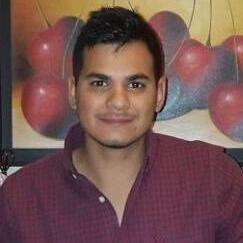
\includegraphics[width=\linewidth]{Foto_CV.png}	%trimming relative to image size

%---------------------------------------------------------------------------------------
%	META SKILLS
%----------------------------------------------------------------------------------------

\cvsection{HABILIDADES}

\cvskill{Python} {5+ yrs} {1} \\[-2pt]

\cvskill{C++} {7+ yrs} {1} \\[-2pt]

\cvskill{MySQL} {5+ yrs} {1} \\[-2pt]

\cvskill{Linux} {5+ yrs} {1} \\[-2pt]

\cvskill{Fortran} {7+ yrs} {1} \\[-2pt]

\cvskill{Django} {5+ yrs} {0.7} \\[-2pt]

\cvskill{Html/CSS} {3+ yrs} {0.7} \\[-2pt]

\cvskill{Javascript} {3+ yrs} {0.8} \\[-2pt]

\cvskill{Microsoft Office} {10+ yrs} {0.8} \\[-2pt]

\cvskill{Visual Basic} {7+ yrs} {0.8} \\[-2pt]

\cvskill{R} {5+ yrs} {1} \\[-2pt]

\cvskill{Matlab} {5+ yrs} {1} \\[-2pt]

\cvskill{GIT} {5+ yrs} {1} \\[-2pt]

\cvsection{CONTACTO}

\icontext{MapMarker}{12}{Hermosillo, Sonora}{black}\\[6pt]
\icontext{MobilePhone}{12}{662-364-8525}{black}\\[6pt]
\iconemail{Envelope}{12}{alan.matzumiya@gmail.com}{alan.matzumiya@gmail.com}{black}\\[6pt]
\iconhref{Github}{12}{github.com/alanmatzumiya}{https://github.com/alanmatzumiya}{black}\\[6pt]


%---------------------------------------------------------------------------------------
%	EDUCATION
%---------------------------------------------------------------------------------------- 
\cvsection{IDIOMAS}

\cvskill{Ingl\'es Oral}{80 \%}{0.8} \\[-2pt]
\cvskill{Ingl\'es Escrito}{90 \%}{0.9} \\[-2pt]

\cvsection{EDUCACI\'ON}

\cvmetaevent
{2011 - 2016}
{Ingenier\'ia Qu\'imica}
{Universidad de Sonora}
{Titulado mediante la presentaci\'on de tesis, la cual se desarroll\'o en el \'area de materiales bajo el tema de: \\
	
\href{http://www.repositorioinstitucional.uson.mx/handle/unison/1840}{\textbf{Caracterizaci\'on y evaluaci\'on de las propiedades bioactivas de una mezcla de biocomp\'ositos de hidroxiapatita/$\beta$-wollastonita preparados por el m\'etodo sol gel: sometidos a tratamientos t\'ermicos diferentes}}.}

\cvmetaevent
{2017 - 2019}
{Maestr\'ia en Ciencias Matem\'aticas}
{Universidad de Sonora}
{El objetivo para obtener este grado fue desarrollar fuertes conocimientos en el \'area del an\'alisis num\'erico, los cuales me permitieron elaborar un trabajo de tesis acerca de los m\'etodos espectrales haciendo uso de las transformadas de Fourier para resolver ecuaciones diferenciales parciales que se presentan en din\'amica de fluidos. Mi trabajo de tesis, junto con los c\'odigos que he desarrollado para entender su implementaci\'on computacional, pueden ser consultados en:

\href{https://github.com/alanmatzumiya/Maestria}{\textbf{github.com/alanmatzumiya}}.}

\vfill\null

%---------------------------------------------------------------------------------------
%	CERTIFICATION
%----------------------------------------------------------------------------------------
  

\end{leftcolumn}
\begin{rightcolumn}
%---------------------------------------------------------------------------------------
%	TITLE  HEADER
%----------------------------------------------------------------------------------------
\fcolorbox{white}{darkcol}{\begin{minipage}[c][3.5cm][c]{1\mpwidth}
	\begin {center}
		\HUGE{ \textbf{ \textcolor{white}{ \uppercase{ Alan Daniel Matzumiya Zazueta } } } } \\[-24pt]
		\textcolor{white}{ \rule{0.1\textwidth}{1.25pt} } \\[4pt]
		\large{ \textcolor{white} {Ingeniero Qu\'imico y Maestro en Ciencias Matem\'aticas.} }
	\end {center}
\end{minipage}} \\[14pt]
\vspace{-12pt}

%---------------------------------------------------------------------------------------
%	PROFILE
%----------------------------------------------------------------------------------------
\vspace{12mm}
\cvsection{Perfil}
\\
\cvtext{\textbf{Edad:} 27 años  \hspace{2mm}  \textbf{Fecha de Nacimiento:} 14/09/1992}
\\\\
\cvtext{\textbf{Lugar de Nacimiento:} Guaymas, Sonora  \hspace{2mm}  \textbf{Estado Civil:} Soltero}
\\\\
\cvtext{La iniciativa es una cualidad con la que puedo ser identificado, la cual me ha motivado para desarrollar de manera autodidacta distintas habilidades y conocimientos s\'olidos en computaci\'on, siendo esta una \'area que me apasiona. \\

Mi gran entusiasmo por el conocimiento, junto con mi trayectoria acad\'emica me ha permitido desarrollar capacidades para resolver problemas matem\'aticos avanzados, dentro y fuera de la ingenier\'a. \\

Obtener experiencia laboral como ingeniero qu\'imico es mi pr\'oxima meta, principalmente en aquellas a\'reas donde pueda ser parte de un equipo de trabajo, y poder explotar mi capacidad de an\'alisis y razonamiento al m\'aximo.  
}

%---------------------------------------------------------------------------------------
%	WORK EXPERIENCE
%----------------------------------------------------------------------------------------
\vspace{5mm}
\cvsection{Experencia Laboral}

\cvevent
{mayo - junio 2015}
{Practicas Profesionales}
{CFE - Central Ciclo Combinado - Hermosillo}
{\cvlist{
		\item Participaci\'on como observador en auditor\'ia ambiental de la planta.
		\item Propuesta de proyecto para modificar planta tratadora de agua, con el fin de resolver un problema de p\'erdidas de presi\'on en las tuber\'ias que transportaban el agua recuperada del proceso de generaci\'on de energ\'ia el\'ectrica, el cual provocaba derrames en un tanque de almacenamiento. 
}}

\newpage
\cvsection{Experiencia Acad\'emica}
\cvevent
{junio 2018}
{Estancia de Investigaci\'on}
{Instituto de Matem\'aticas, UNAM - Oaxaca de Ju\'arez}
{\cvlist{
		\item El objetivo de esta estancia, dirigida por el Dr. Francisco Javier Delgado Vences, fue estudiar unos m\'etodos que demuestran ser muy eficientes para la resoluci\'on de ecuaciones diferenciales parciales estoc\'asticas, los cuales fueron una clave importante para el desarrollo de mi trabajo de tesis. 
		\item Al finalizar, escrib\'i un c\'odigo computacional muy eficiente, el cual puede ser consultado en \url
		{https://github.com/alanmatzumiya/Paper}, con la finalidad de publicar un art\'iculo cient\'ifico acerca de los m\'etodos estudiados, y que fue aprobado y publicado con el t\'itulo de: \\ \href{https://www.researchgate.net/publication/334330862_INITIAL_CONDITIONS_CONTINUITY_OF_A_NUMERICAL_APPROXIMATION_FOR_KOLMOGOROV_EQUATIONS}{\textbf{INITIAL CONDITIONS CONTINUITY OF A NUMERICAL APPROXIMATION FOR KOLMOGOROV EQUATIONS.}}
}}

\vfill\null
\cvevent
{2017-2019}
{Cursos de Programaci\'on en Python}
{Universida de Sonora}
{\cvlist{
		\item El Dr. Abraham Rogelio M\'artin Garc\'ia, actualmente coordinador del posgrado en ciencias de la ingenier\'ia, me invito en tres ocasiones consecutivas para impartir cursos de programaci\'on en el lenguaje Python dirigido a los alumnos de ingenier\'ia, siendo esta una gran experiencia tanto personal y acad\'emica, ya que es un conocimiento que me apasiona transmitir.  
}}

\\

\cvsection{Experiencia Personal}

\cvtext{Mi inter\'es por implementar los conocimientos adquiridos en ingenier\'ia qu\'imica me motivo a tener la iniciativa para experimentar con un equipo de destilaci\'on propio, diseñado para separar etanol producido a partir de la fermentaci\'on de frutas con altos contenidos de az\'ucar. Con este equipo, y con ayuda de un sistema de enfriamiento de tiro inducido que logre construir haciendo uso de mis conocimientos, me permiti\'o obtener sin problemas alcohol con un $90$ \% de pureza. Esta experiencia me ha permitido entender con m\'as detalle estos procesos, que en ingenier\'ia qu\'imica son conocidos como operaciones unitarias.} 

% hotfixes to create fake-space to ensure the whole height is used
\mbox{}
\vfill
\mbox{}
\vfill
\mbox{}
\vfill
\end{rightcolumn}
\end{paracol}
\end{document}

